% Preamble
\documentclass[11pt]{article}

% Packages
\usepackage{amsmath}
\usepackage[a4paper, margin=0.5in]{geometry}
\usepackage{graphicx}
\usepackage[utf8]{inputenc}
\usepackage[T1]{fontenc}
\usepackage[polish]{babel}
\usepackage{float}
\usepackage{hyperref}
\usepackage{cleveref}

\title{Projekt 2. Promethee/Electre}
\author{Oskar Kiliańczyk 151863 \& Wojciech Kot 151876}
\date{}

% Document
\begin{document}

\maketitle
\newpage

\section{Zbiór danych}
\subsection{Jaka jest domena problemu?}
Zbiór danych odzwierciedla rzeczywiste działania rolnictwa z wykorzystaniem czujników $IoT$ i danych satelitarnych. Zawiera informacje o czynnikach środowiskowych i operacyjnych, które wpływają na plony w 500 gospodarstwach rolnych zlokalizowanych m.in. w Indiach, USA i Afryce.

\subsection{Jakie jest źródło danych?}
Dane pochodzą ze zbioru udostępnionego na platformie Kaggle \textit{Smart Farming Sensor Data for Yield Prediction}, autor: Atharva Soundankar. Dostępny pod linkiem: \url{https://www.kaggle.com/datasets/atharvasoundankar/smart-farming-sensor-data-for-yield-prediction}

\subsection{Jaki jest punkt widzenia decydenta?}
Decydent chce maksymalizować zyski ze sprzedaży, co za tym idzie jak najbardziej wspierać wzrost roślin wedle swoich preferencji. Dokładne preferencje zostaną opisane w kolejnym pytaniu.

\subsection{Ile wariantów decyzyjnych zostało uwzględnionych? Czy w oryginalnym zbiorze danych było ich więcej?}
W zbiorze znajduje się $500$ wariantów decyzyjnych. Jednak dla prostoty i wizualizacji ich rankingu na wykresach zdecydowano się na wylosowanie ze znanym ziarnem losowania $10$ wariantów.

\subsection{Opisz jeden z rozważanych wariantów decyzyjnych (podaj jego nazwę, oceny oraz określ preferencje dla tego wariantu).}
Jeden z wylosowanych wariantów jest identyfikowany jako \texttt{FARM0500}.
\begin{table}[H]
\centering
\begin{tabular}{|c||c|c|c|c|}
\hline
\textbf{Wariant} & \textbf{Opady [mm]} & \textbf{Nasłonecznienie [h]} & \textbf{Pestycydy [ml]} & \textbf{Plon [kg/ha]} \\
\hline
FARM0500 & 72.61 & 5.09 & 19.37 & 5891.40 \\
\hline
\end{tabular}
\caption{Oceny kryterialne dla wariantu FARM0500}
\end{table}
Biorąc pod uwagę ten wariant można zauważyć bardzo wysoki wynik dla ilości plonów. Jednakże mimo tego wyniku, każdy inny czynnik jest słaby lub przeciętny. Rozważając wagi decydenta zaobserwować będzie można, że czynnik krótkiego czasu nasłonecznienia, niewielkich opadów nie powinien mu dać znacznej przewagi nad innymi wariantami. Jednak nie można bagatelizować ilości zebranych plonów, które na pewno pomogą mu zająć nie najniższe pozycje.

\subsection{Ile kryteriów zostało uwzględnionych? Czy w oryginalnym zbiorze danych było ich więcej?}
Decydent uwzględnił 4 kryteria. Są to:
\begin{itemize}
    \item \texttt{rainfall\_mm} --– całkowita ilość opadów (w milimetrach),
    \item \texttt{sunlight\_hours} –-- średnia liczba godzin nasłonecznienia na dzień,
    \item \texttt{pesticide\_usage\_ml} –-- dzienne zużycie pestycydów (w mililitrach),
    \item \texttt{yield\_kg\_per\_hectare} –-- plony (w kilogramach na hektar).
\end{itemize}
W oryginalnym zbiorze, było więcej takich kryteriów (22 kolumny, z czego 2 z nich do identyfikacji unikalnego pola).

\subsection{Jakie są dziedziny poszczególnych kryteriów (dyskretne / ciągłe)? Uwaga: w przypadku dziedzin ciągłych określ zakres zmienności kryterium, w innych przypadkach podaj możliwe wartości. Jaki jest charakter poszczególnych kryteriów (zysk / koszt)?}
Zakresy wartości dla kryteriów w zbiorze danych:
\begin{table}[H]
\centering
\begin{tabular}{|c||c|c|c|}
\hline
\textbf{Kryterium} & \textbf{Minimum} & \textbf{Maksimum} & \textbf{Typ} \\
\hline
Opady [mm] & 50.17 & 298.96 & Zysk \\ \hline
Nasłonecznienie [h] & 4.01 & 10.00 & Zysk \\ \hline
Zużycie pestycydów [ml] & 5.05 & 49.94 & Koszt \\ \hline
Plon [kg/ha] & 2023.56 & 5998.29 & Zysk \\
\hline
\end{tabular}
\caption{Zakresy wartości (min–max) dla poszczególnych kryteriów}
\end{table}
Wszystkie kryteria są ciągłe.

\subsection{Czy wszystkie kryteria mają jednakowe znaczenie (czy powinny mieć takie same „wagi”)? Jeśli nie, czy względne znaczenie kryteriów można wyrazić za pomocą wag? W takim przypadku oszacuj wagi każdego kryterium w skali od 1 do 10. Czy wśród kryteriów są takie, które są całkowicie lub prawie nieistotne?}
Kryteria mają swoje wagi. Nie są one tak samo ważne dla decydenta. Decydent wybrał następujące wagi:
\begin{table}[H]
\centering
\begin{tabular}{|c||c|c|c|c|}
\hline
 & \textbf{Opady [mm]} & \textbf{Nasłonecznienie [h]} & \textbf{Zużycie pestycydów [ml]} & \textbf{Plon [kg/ha]} \\
\hline
\textbf{Waga (k)} & 2 & 4 & 2 & 3 \\
\hline
\end{tabular}
\caption{Wagi przypisane do wybranych kryteriów}
\end{table}
Preferuje on średnią dużą ilość słońca, która według niego wpływa znacząco na wzrost roślin. Ważnym kryterium jest również naturalnie ilość zebranych plonów, bo bezpośrednio wpływa to na sprzedaż. Opady oraz zużycie pestycydów zostały wycenione na wagę równą 2. Kryteria nie są bardzo ,,rozrzucone'' a raczej mają podobne (bliskie sobie) wagi. 

\subsection{Czy w rozważanym zbiorze danych występują zdominowane warianty decyzyjne? Jeśli tak, przedstaw wszystkie (warianty dominujące i zdominowane), podając ich nazwy oraz wartości dla poszczególnych kryteriów.}
Rozpatrywany zbiór według danego ziarna losowania:
\begin{table}[H]
\centering
\begin{tabular}{|c||c|c|c|c|}
\hline
\textbf{Farm ID} & \textbf{Opady [mm]} & \textbf{Nasłonecznienie [h]} & \textbf{Pestycydy [ml]} & \textbf{Plon [kg/ha]} \\
\hline
FARM0500 & 72.61 & 5.09 & 19.37 & 5891.40 \\ \hline
FARM0269 & 172.48 & 4.11 & 33.14 & 5247.57 \\ \hline
FARM0025 & 237.74 & 4.64 & 12.91 & 2200.87 \\ \hline
FARM0328 & 256.34 & 6.71 & 47.54 & 5535.92 \\ \hline
FARM0015 & 129.04 & 4.44 & 49.93 & 2852.62 \\ \hline
FARM0483 & 135.54 & 8.42 & 18.03 & 3715.81 \\ \hline
FARM0046 & 259.37 & 7.96 & 29.24 & 5051.49 \\ \hline
FARM0433 & 65.99 & 8.85 & 44.57 & 2156.34 \\ \hline
FARM0346 & 230.53 & 6.96 & 25.56 & 5904.72 \\ \hline
FARM0384 & 219.67 & 6.93 & 5.86  & 2254.04 \\
\hline
\end{tabular}
\caption{Warianty decyzyjne i ich wartości dla poszczególnych kryteriów}
\end{table}

Poszukiwano parami, silnej dominacji. W danym zbiorze znaleziono następujące:
\begin{table}[H]
\centering
\begin{tabular}{|c||c|c|c|c|}
\hline
\textbf{Farm ID} & \textbf{Opady [mm] (zysk)} & \textbf{Nasł. [h] (zysk)} & \textbf{Pestycydy [ml] (koszt)} & \textbf{Plon [kg/ha] (zysk)} \\
\hline
FARM0328 & 256.34 & 6.71 & 47.54 & 5535.92 \\ \hline
FARM0015 & 129.04 & 4.44 & 49.93 & 2852.62 \\
\hline
\end{tabular}
\caption{Dominacja: FARM0328 $\succ$ FARM0015}
\end{table}

\begin{table}[H]
\centering
\begin{tabular}{|c||c|c|c|c|}
\hline
\textbf{Farm ID} & \textbf{Opady [mm] (zysk)} & \textbf{Nasł. [h] (zysk)} & \textbf{Pestycydy [ml] (koszt)} & \textbf{Plon [kg/ha] (zysk)} \\
\hline
FARM0483 & 135.54 & 8.42 & 18.03 & 3715.81 \\ \hline
FARM0015 & 129.04 & 4.44 & 49.93 & 2852.62 \\
\hline
\end{tabular}
\caption{Dominacja: FARM0483 $\succ$ FARM0015}
\end{table}

\begin{table}[H]
\centering
\begin{tabular}{|c||c|c|c|c|}
\hline
\textbf{Farm ID} & \textbf{Opady [mm] (zysk)} & \textbf{Nasł. [h] (zysk)} & \textbf{Pestycydy [ml] (koszt)} & \textbf{Plon [kg/ha] (zysk)} \\
\hline
FARM0046 & 259.37 & 7.96 & 29.24 & 5051.49 \\ \hline
FARM0015 & 129.04 & 4.44 & 49.93 & 2852.62 \\
\hline
\end{tabular}
\caption{Dominacja: FARM0046 $\succ$ FARM0015}
\end{table}

\begin{table}[H]
\centering
\begin{tabular}{|c||c|c|c|c|}
\hline
\textbf{Farm ID} & \textbf{Opady [mm] (zysk)} & \textbf{Nasł. [h] (zysk)} & \textbf{Pestycydy [ml] (koszt)} & \textbf{Plon [kg/ha] (zysk)} \\
\hline
FARM0346 & 230.53 & 6.96 & 25.56 & 5904.72 \\ \hline
FARM0269 & 172.48 & 4.11 & 33.14 & 5247.57 \\
\hline
\end{tabular}
\caption{Dominacja: FARM0346 $\succ$ FARM0269}
\end{table}

\begin{table}[H]
\centering
\begin{tabular}{|c||c|c|c|c|}
\hline
\textbf{Farm ID} & \textbf{Opady [mm] (zysk)} & \textbf{Nasł. [h] (zysk)} & \textbf{Pestycydy [ml] (koszt)} & \textbf{Plon [kg/ha] (zysk)} \\
\hline 
FARM0346 & 230.53 & 6.96 & 25.56 & 5904.72 \\ \hline
FARM0015 & 129.04 & 4.44 & 49.93 & 2852.62 \\
\hline
\end{tabular}
\caption{Dominacja: FARM0346 $\succ$ FARM0015}
\end{table}

\subsection{Jak według Ciebie powinien wyglądać teoretycznie najlepszy wariant decyzyjny? Czy powinien mieć niewielką przewagę w wielu kryteriach, czy raczej silną przewagę w kilku (ale kluczowych) kryteriach? Których?}
Najlepszy wariant decyzyjny powinien osiągać najlepsze (tj. najwyższe) wyniki na kryteriach nasłonecznienia i ilości zebranych plonów. Dominacja na obu z tych kryteriów powinna dać wystarczającą przewagę nawet przy słabej ocenie na pozostałych dwóch kryteriach o niższych wagach.

\subsection{Który z rozważanych wariantów decyzyjnych (podaj nazwę i wartości dla poszczególnych kryteriów) wydaje się najlepszy / zdecydowanie lepszy od pozostałych? Czy decyduje o tym jeden czynnik (np. zdecydowanie najniższa cena), czy raczej ogólna wartość kryteriów? Czy ten wariant ma jakieś słabe strony?}
Wybrano kilka dobrze rokujących wariantów:
\begin{table}[H]
\centering
\begin{tabular}{|c||c|c|c|c|}
\hline
\textbf{Farm ID} & \textbf{Opady [mm] (zysk)} & \textbf{Nasł. [h] (zysk)} & \textbf{Pestycydy [ml] (koszt)} & \textbf{Plon [kg/ha] (zysk)} \\
\hline
FARM0046 & 259.37 & 7.96 & 29.24 & 5051.49 \\
\hline
FARM0346 & 230.53 & 6.96 & 25.56 & 5904.72 \\
\hline
FARM0500 & 72.61 & 5.09 & 19.37 & 5891.40 \\
\hline
\end{tabular}
\caption{Porównanie najlepszych (według decydenta) wariantów decyzyjnych}
\end{table}

Podane przykłady reprezentują założenie decydenta. Wysoki wynik na nasłonecznieniu oraz zbiorach plonów co jest preferowane (ma najwyższe wagi). Nasłonecznienie jest jak $4:3$ w skali do ilości plonów stąd, powątpiewam w to, że $FARM0500$ nadrobi swoim wynikiem na zbiorach plonów około $2-3$ godzin nasłonecznienia. Pierwsze dwa warianty mają dużą liczbę opadów, liczne plony oraz bardzo długi czas średniego nasłonecznienia dziennego co powinno dać im osiągnąć wysokie wyniki.

\subsection{Który z rozważanych wariantów decyzyjnych (podaj nazwę i wartości dla poszczególnych kryteriów) wydaje się najgorszy / zdecydowanie gorszy od pozostałych? Czy decyduje o tym jeden czynnik (np. zdecydowanie najwyższa cena), czy raczej ogólna wartość kryteriów? Czy ten wariant ma jakieś mocne strony?}
To co można już zaobserwować z samej analizy dominacji, czyli wariant $FARM0015$:
\begin{table}[H]
\centering
\caption{Charakterystyka wariantu FARM0015 (kolumny jako kryteria)}
\begin{tabular}{|c||c|c|c|c|}
\hline
\textbf{Farm ID} & \textbf{Opady [mm] (zysk)} & \textbf{Nasł. [h] (zysk)} & \textbf{Pestycydy [ml] (koszt)} & \textbf{Plon [kg/ha] (zysk)} \\
\hline
FARM0015 & 129.04 & 4.44 & 49.93 & 2852.62 \\
\hline
\end{tabular}
\end{table}

Wariant cechuje się bardzo niskim czasem nasłonecznienie (praktycznie minimalnym), dużym zużyciem pestycydów (prawie maksymalnym) oraz niewielką liczbą plonów. Ilość opadów jest przeciętna, raczej gorsza niż lepsza. Połączenie tych wszystkich kryteriów daje jasny obraz, dlaczego ten wariant jest zdominowany przez wiele innych. Nie ma on żadnej mocnej strony.

\subsection{Podaj co najmniej 4 porównania parami pomiędzy wariantami w Twoim zbiorze danych.}
\begin{table}[H]
\centering
\begin{tabular}{|c||c|c|c|}
\hline
\textbf{Kryterium} & \textbf{FARM0328} & \textbf{FARM0015} & \textbf{Preferowany} \\
\hline
Opady [mm] (zysk)           & 256.34 & 129.04 & FARM0328 \\ \hline
Nasłonecznienie [h] (zysk) & 6.71   & 4.44   & FARM0328 \\ \hline
Pestycydy [ml] (koszt)     & 47.54  & 49.93  & FARM0328 \\ \hline
Plon [kg/ha] (zysk)       & 5535.92& 2852.62& FARM0328 \\
\hline
\end{tabular}
\caption{Porównanie FARM0328 vs FARM0015}
\end{table}
Znane już porównanie --- $FARM0328$ dominuje $FARM0015$ we wszystkich kryteriach, w tym znacząco w plonach.

\begin{table}[H]
\centering
\begin{tabular}{|c||c|c|c|}
\hline
\textbf{Kryterium} & \textbf{FARM0346} & \textbf{FARM0269} & \textbf{Preferowany} \\
\hline
Opady [mm] (zysk)           & 230.53 & 172.48 & FARM0346 \\ \hline
Nasłonecznienie [h] (zysk) & 6.96   & 4.11   & FARM0346 \\ \hline
Pestycydy [ml] (koszt)      & 25.56  & 33.14  & FARM0346 \\ \hline
Plon [kg/ha] (zysk)        & 5904.72& 5247.57& FARM0346 \\
\hline
\end{tabular}
\caption{Porównanie FARM0346 vs FARM0269}
\end{table}
Kolejne znane porównanie --- $FARM0346$ ma lepsze wyniki we wszystkich kryteriach w porównaniu do $FARM0269$.

\begin{table}[H]
\centering
\begin{tabular}{|c||c|c|c|}
\hline
\textbf{Kryterium} & \textbf{FARM0046} & \textbf{FARM0384} & \textbf{Preferowany} \\
\hline
Opady [mm] (zysk)           & 259.37 & 219.67 & FARM0046 \\ \hline
Nasłonecznienie [h] (zysk) & 7.96   & 6.93   & FARM0046 \\ \hline
Pestycydy [ml] (koszt)      & 29.24  & 5.86   & FARM0384 \\ \hline
Plon [kg/ha] (zysk)        & 5051.49& 2254.04& FARM0046 \\
\hline
\end{tabular}
\caption{Porównanie FARM0046 vs FARM0384}
\end{table}
$FARM0046$ wygrywa w trzech kryteriach, ale $FARM0384$ zużywa znacznie mniej pestycydów --- nie powinno to mieć większego znaczenia ponieważ pestycydy mają stosunkowo niską wagę w porównaniu np. do ponad dwukrotnej przewagi w ilości plonów.

\begin{table}[H]
\centering
\begin{tabular}{|c||c|c|c|}
\hline
\textbf{Kryterium} & \textbf{FARM0483} & \textbf{FARM0500} & \textbf{Preferowany} \\
\hline
Opady [mm] (zysk)           & 135.54 & 72.61  & FARM0483 \\ \hline
Nasłonecznienie [h] (zysk) & 8.42   & 5.09   & FARM0483 \\ \hline
Pestycydy [ml] (zysk)      & 18.03  & 19.37  & FARM0483 \\ \hline
Plon [kg/ha] (zysk)        & 3715.81& 5891.40& FARM0500 \\
\hline
\end{tabular}
\caption{Porównanie FARM0483 vs FARM0500}
\end{table}
$FARM0483$ lepszy w trzech kryteriach, ale $FARM0500$ osiąga znacznie wyższy plon. Różnica w nasłonecznieniu (około 3.5 godziny) również będzie miała tutaj duże znaczenie w wyniku końcowym.

\section{Promethee} \label{sec:Promethee}
\subsection{Opisz informacje preferencyjną podaną na wejściu metod}
W oparciu o min-max podanych kryterium decydent wybrał następujące progi i wagi:
\begin{table}[H]
\centering
\begin{tabular}{|c||c|c|c|c|c|}
\hline
\textbf{Kryterium} & \textbf{q} & \textbf{p} & \textbf{v} & \textbf{Waga (k)} & \textbf{Typ} \\
\hline
Nasłonecznienie [h]            & 0.3   & 0.8   & 2.0   & 4 & zysk \\ \hline
Zużycie pestycydów [ml]        & 2     & 6     & 15    & 2 & koszt \\ \hline
Opady [mm]                     & 10    & 25    & 70    & 2 & zysk \\ \hline
Plon [kg/ha]                   & 150   & 500   & 1500  & 3 & zysk \\
\hline
\end{tabular}
\caption{Przyjęte wartości progowe (q, p, v), wagi oraz typy dla każdego z kryteriów.}
\end{table}

\subsection{Podaj ostateczny wynik uzyskany za pomocą metod}
Metody Promethee wyliczyły następujące przepływy dla naszego zbioru danych:
\begin{table}[H]
\centering
\begin{tabular}{|c||c|c|c|}
\hline
\textbf{ID Farmy} & \textbf{Przepływ pozytywny} & \textbf{Przepływ negatywny} & \textbf{Przepływ netto} \\
\hline
FARM0500 & 3.523751 & 4.363636 & -0.839886 \\ \hline
FARM0269 & 3.399543 & 4.834169 & -1.434626 \\ \hline
FARM0025 & 3.512000 & 3.726788 & -0.214788 \\ \hline
FARM0328 & 5.230976 & 2.192881 &  3.038095 \\ \hline
FARM0015 & 1.556364 & 6.479545 & -4.923182 \\ \hline
FARM0483 & 4.240000 & 3.916364 &  0.323636 \\ \hline
FARM0046 & 6.095576 & 1.885592 &  4.209984 \\ \hline
FARM0433 & 1.698636 & 6.090909 & -4.392273 \\ \hline
FARM0346 & 5.449524 & 2.000000 &  3.449524 \\ \hline
FARM0384 & 4.181818 & 3.398303 &  0.783515 \\
\hline
\end{tabular}
\caption{Zestawienie przepływów pozytywnych, negatywnych i netto dla wszystkich wariantów.}
\end{table}

Dzięki nim jesteśmy w stanie uzyskać wyniki dla \textit{Promethee I} oraz \textit{Promethee II}.
\subsubsection{Promethee I}
Dzięki przepływom dodatnim i ujemnym możemy stworzyć ranking cząstkowy:
\begin{table}[H]
\centering
\begin{tabular}{|c||c|c|c|c|c|c|c|c|c|c|}
\hline
\textbf{ID Farmy} & \textbf{F0500} & \textbf{F0269} & \textbf{F0025} & \textbf{F0328} & \textbf{F0015} & \textbf{F0483} & \textbf{F0046} & \textbf{F0433} & \textbf{F0346} & \textbf{F0384} \\
\hline
F0500 & 1 & 1 & 0 & 0 & 1 & 0 & 0 & 1 & 0 & 0 \\
\hline
F0269 & 0 & 1 & 0 & 0 & 1 & 0 & 0 & 1 & 0 & 0 \\
\hline
F0025 & 0 & 1 & 1 & 0 & 1 & 0 & 0 & 1 & 0 & 0 \\
\hline
F0328 & 1 & 1 & 1 & 1 & 1 & 1 & 0 & 1 & 0 & 1 \\
\hline
F0015 & 0 & 0 & 0 & 0 & 1 & 0 & 0 & 0 & 0 & 0 \\
\hline
F0483 & 1 & 1 & 0 & 0 & 1 & 1 & 0 & 1 & 0 & 0 \\
\hline
F0046 & 1 & 1 & 1 & 1 & 1 & 1 & 1 & 1 & 1 & 1 \\
\hline
F0433 & 0 & 0 & 0 & 0 & 1 & 0 & 0 & 1 & 0 & 0 \\
\hline
F0346 & 1 & 1 & 1 & 1 & 1 & 1 & 0 & 1 & 1 & 1 \\
\hline
F0384 & 1 & 1 & 1 & 0 & 1 & 0 & 0 & 1 & 0 & 1 \\
\hline
\end{tabular}
\caption{Ranking cząstkowy wariantów decyzyjnych na podstawie Promethee I.}
\end{table}

\begin{figure}[H]
	\centering
	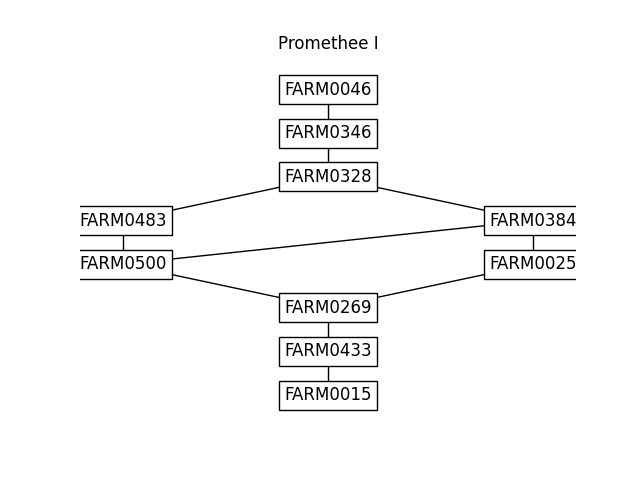
\includegraphics[scale=0.75]{output/Promethee I.png}
	\caption{Wynikowy wykres dla metody Promethee I}
\end{figure}

\subsubsection{Promethee II}
Dzięki przepływowi netto możemy stworzyć ranking zupełny:
\begin{table}[H]
\centering
\begin{tabular}{|c||c|c|c|c|c|c|c|c|c|c|}
\hline
\textbf{ID Farmy} & \textbf{F0500} & \textbf{F0269} & \textbf{F0025} & \textbf{F0328} & \textbf{F0015} & \textbf{F0483} & \textbf{F0046} & \textbf{F0433} & \textbf{F0346} & \textbf{F0384} \\
\hline
F0500 & 1 & 1 & 0 & 0 & 1 & 0 & 0 & 1 & 0 & 0 \\
\hline
F0269 & 0 & 1 & 0 & 0 & 1 & 0 & 0 & 1 & 0 & 0 \\
\hline
F0025 & 1 & 1 & 1 & 0 & 1 & 0 & 0 & 1 & 0 & 0 \\
\hline
F0328 & 1 & 1 & 1 & 1 & 1 & 1 & 0 & 1 & 0 & 1 \\
\hline
F0015 & 0 & 0 & 0 & 0 & 1 & 0 & 0 & 0 & 0 & 0 \\
\hline
F0483 & 1 & 1 & 1 & 0 & 1 & 1 & 0 & 1 & 0 & 0 \\
\hline
F0046 & 1 & 1 & 1 & 1 & 1 & 1 & 1 & 1 & 1 & 1 \\
\hline
F0433 & 0 & 0 & 0 & 0 & 1 & 0 & 0 & 1 & 0 & 0 \\
\hline
F0346 & 1 & 1 & 1 & 1 & 1 & 1 & 0 & 1 & 1 & 1 \\
\hline
F0384 & 1 & 1 & 1 & 0 & 1 & 1 & 0 & 1 & 0 & 1 \\
\hline
\end{tabular}
\caption{Ranking zupełny wariantów decyzyjnych na podstawie Promethee II.}
\end{table}

\begin{figure}[H]
	\centering
	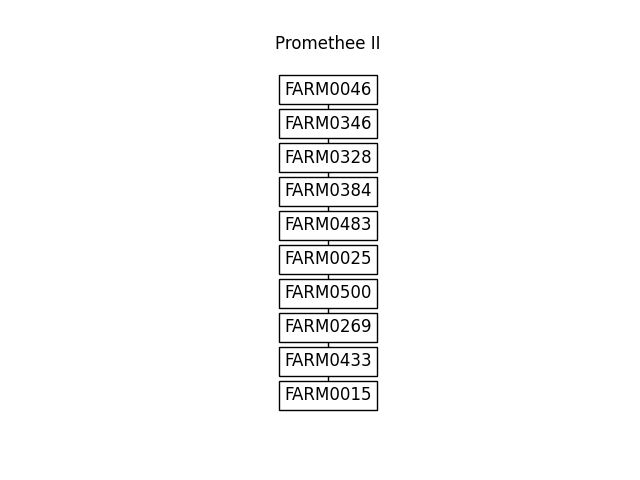
\includegraphics[scale=0.75]{output/Promethee II.png}
	\caption{Wynikowy wykres dla metody Promethee II}
\end{figure}

\subsection{Porównaj ranking cząstkowy i zupełny (Promethee I i Promethee II)}
Oba rankingi są podobne do siebie. Ranking cząstkowy dopuszcza nieporównywalności wariantów w przypadku różnic w przepływach ujemnych i dodatnich. Daje lepszy pogląd na to, że niektóre warianty są skrajne w stosunku do siebie lub różnią się na tyle (według progów decydenta), że nie można ich rozpatrywać jednakowo. Ranking zupełny, stosujący przepływ netto, nie ma takich rozróżnień i ustawia ranking według przepływu netto właśnie. Można zaobserwować, że wyniki na górze i na dole rankingu nie zmieniły się w zależności od metody, zaś nieporównywalne warianty środkowe zostały ustawione według wartości ich przepływu netto.

\subsection{Porównaj wyniki uzyskane za pomocą zaimplementowanej metody z wariantami, które zidentyfikowałeś jako najlepszą i najgorszą (w sekcji Zbiór danych)}
W sekcji ,,Zbiór danych'' zidentyfikowaliśmy warianty $FARM0046$ oraz $FARM0346$ jako najlepsze (wariant $FARM0500$ mimo wyróżnienia był poddany w wątpliwość), zaś jako najgorszy wariant $FARM0015$ ze względu na bycie zdominowanym przez większość wariantów ze zbioru. W obu rankingach najlepsze warianty uznane przez nas okazały się również najlepsze w rankingach, za to wariant najgorszy faktycznie też został określony jako najgorszy. Wariant $FARM0500$ jednak pomimo dobrych ocen i naszej wyceny został oceniony raczej gorzej i umiejscawia się w drugiej połowie rankingów.

\subsection{Porównaj wyniki uzyskane za pomocą zaimplementowanej metody z wcześniejszymi przekonaniami na temat wariantów (porównania parami określone w sekcji Zbiór danych)}
W sekcji ,,Zbiór danych'' porównywaliśmy ze sobą następujące warianty:
\begin{itemize}
\item $FARM0328$ --- $FARM0015$ --- relacja dominacji, a więc nic dziwnego, oba rankingi zachowały tą relację,
\item $FARM0346$ --- $FARM0269$ --- kolejny przypadek relacji dominacji, jednak nie tak drastycznej, rankingi zachowały relację ustawiając $FARM0346$ na pozycji 2 w rankingu, zaś drugi wariant dopiero 3 od końca w obu przypadkach,
\item $FARM0046$ --- $FARM0384$ --- najlepszy wariant wygrywa z $FARM0384$. Wygrywał na 3 wariantach, przegrywając tylko na ilości pestycydów zużywanych (czyli mało znaczącym w skali problemu czynniku), co też zauważyliśmy wcześniej,
\item $FARM0483$ --- $FARM0500$ --- mimo przewagi pierwszego wariantu aż na trzech kryteriach były one bardzo blisko siebie w rankingach. Tak jak zauważyliśmy znacznie wyższe wyniki dla zbioru plonów o wysokiej wadze dla $FARM0500$ dały tutaj bardzo dużo pomimo strat na innych polach. Różnica w nasłonecznieniu dała zwycięstwo wariantowi $FARM0483$ w obu rankingach. Warto zauważyć, że dla \textit{Promethee I} są one oddalone o 1 poziom będąc nieporównywalne z $FARM0025$.
\end{itemize}

\subsection{Dodatkowe uwagi na temat uzyskanych wyników. Możesz odnieść się m.in. do wariantów, które cię zaskoczyły, lub do pozycji w rankingu, które uważasz za niepoprawne.}
Zaskoczyliśmy się pozycjonowaniem wariantu $FARM0500$ w rankingach. Pomimo problemów na innych kryteriach, spodziewaliśmy się, że bardzo wysoki wynik na zebranych plonach usytuuje go wyżej w rankingu. Jednak wagi zostały dobrane w taki sposób, że nie dało mu to znaczącej przewagi i opłacało się mieć ,,przeciętne'' i lepsze wyniki na wielu kryteriach niż tylko na jednym znaczącym. To samo tyczy się wariantu $FARM0433$, który ma rewelacyjny wynik jeśli chodzi o nasłonecznienie ($8.85$ --- najwyższy dla tego zbioru). Jednakże braki w zbiorach plonów oraz bardzo niewielkie opady skutecznie go umiejscowiły na przedostatniej pozycji w rankingu.

\section{Electre III}
\subsection{Opisz informacje preferencyjne podane na wejściu metody}
\textbf{Uwaga} to samo zostało opisane w sekcji ~\ref{sec:Promethee}.

W oparciu o min-max podanych kryterium decydent wybrał następujące progi i wagi:
\begin{table}[H]
\centering
\begin{tabular}{|c||c|c|c|c|c|}
\hline
\textbf{Kryterium} & \textbf{q} & \textbf{p} & \textbf{v} & \textbf{Waga (k)} & \textbf{Typ} \\
\hline
Nasłonecznienie [h]            & 0.3   & 0.8   & 2.0   & 4 & zysk \\ \hline
Zużycie pestycydów [ml]        & 2     & 6     & 15    & 2 & koszt \\ \hline
Opady [mm]                     & 10    & 25    & 70    & 2 & zysk \\ \hline
Plon [kg/ha]                   & 150   & 500   & 1500  & 3 & zysk \\
\hline
\end{tabular}
\caption{Przyjęte wartości progowe (q, p, v), wagi oraz typy dla każdego z kryteriów.}
\end{table}

\subsection{Podaj ostateczny wynik uzyskany za pomocą metody}
Metoda \textit{Electre III} uzyskała następujące wyniki:
\subsubsection{Destylacja schodząca}
\begin{table}[H]
\centering
\begin{tabular}{|c||c|c|c|c|c|c|c|c|c|c|}
\hline
\textbf{ID Farmy} & \textbf{F0500} & \textbf{F0269} & \textbf{F0025} & \textbf{F0328} & \textbf{F0015} & \textbf{F0483} & \textbf{F0046} & \textbf{F0433} & \textbf{F0346} & \textbf{F0384} \\
\hline
F0500 & 1 & 1 & 1 & 0 & 1 & 0 & 0 & 1 & 0 & 0 \\
\hline
F0269 & 1 & 1 & 1 & 0 & 1 & 0 & 0 & 1 & 0 & 0 \\
\hline
F0025 & 1 & 1 & 1 & 0 & 1 & 0 & 0 & 1 & 0 & 0 \\
\hline
F0328 & 1 & 1 & 1 & 1 & 1 & 1 & 0 & 1 & 0 & 0 \\
\hline
F0015 & 0 & 0 & 0 & 0 & 1 & 0 & 0 & 1 & 0 & 0 \\
\hline
F0483 & 1 & 1 & 1 & 1 & 1 & 1 & 0 & 1 & 0 & 0 \\
\hline
F0046 & 1 & 1 & 1 & 1 & 1 & 1 & 1 & 1 & 1 & 1 \\
\hline
F0433 & 0 & 0 & 0 & 0 & 1 & 0 & 0 & 1 & 0 & 0 \\
\hline
F0346 & 1 & 1 & 1 & 1 & 1 & 1 & 0 & 1 & 1 & 1 \\
\hline
F0384 & 1 & 1 & 1 & 1 & 1 & 1 & 0 & 1 & 0 & 1 \\
\hline
\end{tabular}
\caption{Destylacja schodząca według metody Electre III.}
\end{table}

\begin{figure}[H]
	\centering
	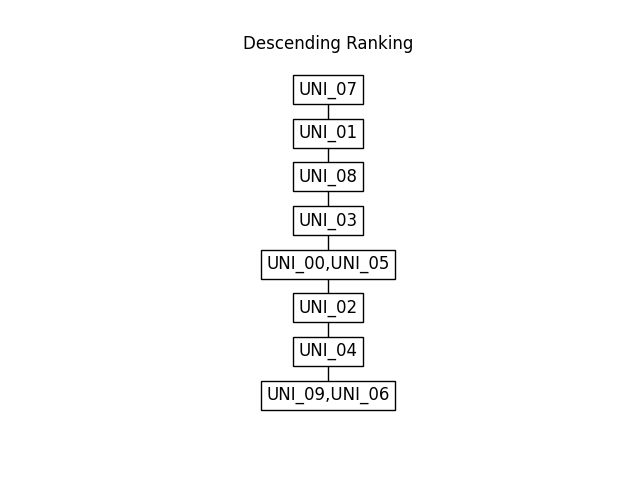
\includegraphics[scale=0.75]{output/Descending Ranking.png}
	\caption{Wynikowy wykres dla metody Electre III destylacji schodzącej}
\end{figure}

\subsubsection{Destylacja wchodząca}
\begin{table}[H]
\centering
\begin{tabular}{|c||c|c|c|c|c|c|c|c|c|c|}
\hline
\textbf{ID Farmy} & \textbf{F0500} & \textbf{F0269} & \textbf{F0025} & \textbf{F0328} & \textbf{F0015} & \textbf{F0483} & \textbf{F0046} & \textbf{F0433} & \textbf{F0346} & \textbf{F0384} \\
\hline
F0500 & 1 & 1 & 1 & 1 & 1 & 1 & 0 & 1 & 0 & 0 \\
\hline
F0269 & 0 & 1 & 0 & 0 & 1 & 0 & 0 & 1 & 0 & 0 \\
\hline
F0025 & 0 & 1 & 1 & 0 & 1 & 0 & 0 & 1 & 0 & 0 \\
\hline
F0328 & 1 & 1 & 1 & 1 & 1 & 1 & 0 & 1 & 0 & 0 \\
\hline
F0015 & 0 & 0 & 0 & 0 & 1 & 0 & 0 & 0 & 0 & 0 \\
\hline
F0483 & 1 & 1 & 1 & 1 & 1 & 1 & 0 & 1 & 0 & 0 \\
\hline
F0046 & 1 & 1 & 1 & 1 & 1 & 1 & 1 & 1 & 1 & 1 \\
\hline
F0433 & 0 & 1 & 0 & 0 & 1 & 0 & 0 & 1 & 0 & 0 \\
\hline
F0346 & 1 & 1 & 1 & 1 & 1 & 1 & 1 & 1 & 1 & 1 \\
\hline
F0384 & 1 & 1 & 1 & 1 & 1 & 1 & 1 & 1 & 1 & 1 \\
\hline
\end{tabular}
\caption{Destylacja wchodząca według metody Electre III.}
\end{table}

\begin{figure}[H]
	\centering
	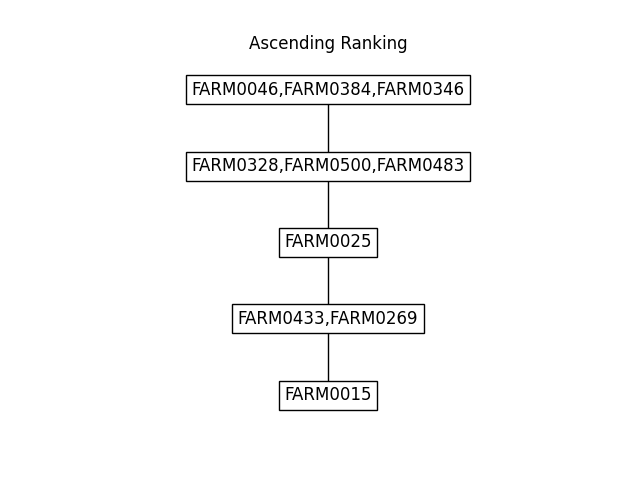
\includegraphics[scale=0.75]{output/Ascending Ranking.png}
	\caption{Wynikowy wykres dla metody Electre III destylacji wchodzącej}
\end{figure}

\subsubsection{Ranking końcowy}
Dzięki wynikom obu destylacji tworzony jest ranking końcowy:
\begin{table}[H]
\centering
\begin{tabular}{|c||c|c|c|c|c|c|c|c|c|c|}
\hline
\textbf{ID Farmy} & \textbf{F0500} & \textbf{F0269} & \textbf{F0025} & \textbf{F0328} & \textbf{F0015} & \textbf{F0483} & \textbf{F0046} & \textbf{F0433} & \textbf{F0346} & \textbf{F0384} \\
\hline
F0500 & 1 & 1 & 1 & 0 & 1 & 0 & 0 & 1 & 0 & 0 \\
\hline
F0269 & 0 & 1 & 0 & 0 & 1 & 0 & 0 & 1 & 0 & 0 \\
\hline
F0025 & 0 & 1 & 1 & 0 & 1 & 0 & 0 & 1 & 0 & 0 \\
\hline
F0328 & 1 & 1 & 1 & 1 & 1 & 1 & 0 & 1 & 0 & 0 \\
\hline
F0015 & 0 & 0 & 0 & 0 & 1 & 0 & 0 & 0 & 0 & 0 \\
\hline
F0483 & 1 & 1 & 1 & 1 & 1 & 1 & 0 & 1 & 0 & 0 \\
\hline
F0046 & 1 & 1 & 1 & 1 & 1 & 1 & 1 & 1 & 1 & 1 \\
\hline
F0433 & 0 & 0 & 0 & 0 & 1 & 0 & 0 & 1 & 0 & 0 \\
\hline
F0346 & 1 & 1 & 1 & 1 & 1 & 1 & 0 & 1 & 1 & 1 \\
\hline
F0384 & 1 & 1 & 1 & 1 & 1 & 1 & 0 & 1 & 0 & 1 \\
\hline
\end{tabular}
\caption{Ranking końcowy według metody Electre III.}
\end{table}

\begin{figure}[H]
	\centering
	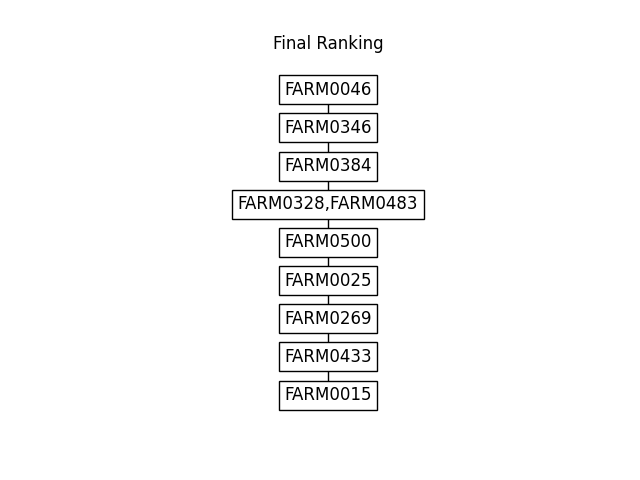
\includegraphics[scale=0.75]{output/Final Ranking.png}
	\caption{Wynikowy wykres dla metody Electre III końcowego rankingu}
\end{figure}

\subsection{Skomentuj ostateczne wyniki metody}

\subsection{Porównaj wyniki uzyskane za pomocą zaimplementowanej metody z wariantami, które zidentyfikowałeś jako najlepszy i najgorszy (w sekcji Zbiór danych)}

\subsection{Porównaj wyniki uzyskane za pomocą zaimplementowanej metody z wcześniejszymi przekonaniami na temat wariantów (porównania parami określone w sekcji Zbiór danych)}

\subsection{Dodatkowe uwagi na temat uzyskanych wyników. Możesz odnieść się m.in. do wariantów, które cię zaskoczyły, lub do pozycji w rankingu, które uważasz za niepoprawne.}

\section{Porównanie}
\subsection{Zgodność między metodami}

\subsection{Różnice między metodami}

\subsection{Dodatkowe uwagi na temat wyników}


\section{Link do repozytorium}\label{sec:link-do-repo}
Kod źródłowy w repozytorium GitHub dostępny pod linkiem: \\
\href{https://github.com/KotZPolibudy/PUT_ISWD/tree/main/projekt2}{Repozytorium ISWD - projekt 2}.


\end{document}
